

\begin{frame}{Mallet}

\begin{itemize}
  \item Developed at UMass Amherst by Andrew McCallum and David Mimno (among others)
  \item Very fast implementation of Gibbs sampling for topic modeling
  \item (Somewhat) friendly interface
  \item Easiest on \textsc{unix}-derived operating systems, but also works on Windows
  \item Requires Java
\end{itemize}

\begin{columns}
\column{.5\linewidth}
\begin{block}{Download Location}
  http://mallet.cs.umass.edu/
\end{block}
\column{.5\linewidth}

\includegraphics[width=.9\linewidth]{topic_models/mallet}
\end{columns}
\end{frame}


\begin{frame}
  \frametitle{Scenario}

  \begin{itemize}
    \item Learn a (small-sized) topic model on \textsc{nih} data
    \item Discover the priorities of \textsc{nih}
    \item Walk through the commands to do everything
  \end{itemize}
\end{frame}

\begin{frame}[fragile]


\frametitle {Getting Your Data}


\begin{itemize}
	\item All data in single directory
	\item Each file is separate document
	\item (Optional) Remove stop words beforehand
\end{itemize}

%\begin{columns}
%  \column{.6\linewidth}
%    \begin{itemize}
%      \item Connect to database
%      \item \alert<1>{First column: doc id}
%      \item \alert<2>{Second column: language}
%      \item \alert<3>{Third column: text}
%    \end{itemize}
%  \column{.3\linewidth}
%     \begin{tabular}{lll}
%       \alert<1>{doc} & \alert<2>{lang} & \alert<3>{text} \\
%     \end{tabular}
%\end{columns}

\begin{block}{Download}
  \url{http://umiacs.umd.edu/~jbg/lda_demo/}
\end{block}

\pause \pause \pause \pause 
\begin{lstlisting}
doc0    none    It is proposed to grow and characterize ternary alloys of ...
doc1    none    This project will focus on development of new cutting tool designs ...
doc2    none    The purpose of the proposed work is to design a novel cooling device ...
doc3    none    The objective of this research project is to develop a wireless ...
\end{lstlisting}

\end{frame}


\begin{frame}[fragile]

  \frametitle{Preparing \textsc{nsf} Data}

  \begin{block}{Mallet Command}
    mallet \alert<2>{import-file} \alert<3>{--remove-stopwords} \alert<4>{--keep-sequence} \alert<5>{--input nsf-30k.txt} \alert<6>{--output nsf.mallet}
  \end{block}

  \pause

  \begin{itemize}
    \item \alert<2>{Tell Mallet what to do}
    \item \alert<3>{Remove words like ``the'', ``and'', ``of''} (otherwise, they'd be at the top of every topic)
    \item \alert<4>{Remember the order of words} (required for Gibbs sampling)
    \item \alert<5>{The input text file}
    \item \alert<6>{Where it writes the binary file}
  \end{itemize}

\end{frame}

%\begin{frame}
%  \frametitle{Preparing \textsc{nrc} data}
%
%  \begin{block}{Mallet Command}
%    mallet import-file --remove-stopwords --keep-sequence --input merged.txt --output nrc.mallet \alert<2>{--use-pipe-from nsf.mallet}
%  \end{block}
%
%  \begin{itemize}
%    \item Nearly identical to previous command
%    \pause
%    \item Main difference: use \textsc{nsf} vocabulary to encode the data
%    \item \textsc{lda} doesn't know what words mean
%    \item Internally, these algorithms map words to numbers: oxygen (2134), neutrino (33), Weber (1701)
%    \item This ensures that this mapping is consistent between datasets
%   \end{itemize}
%
%\end{frame}


\begin{frame}
  \frametitle{Fitting a topic model}

\begin{block}{Mallet Command}
\small
  mallet train-topics --input \alert<2>{nsf.mallet}  --num-topics \alert<3>{10} --num-iterations \alert<4>{100} --output-model \alert<5>{nsf\_10.model} --output-state \alert<6>{nsf\_10.state.gz} --output-doc-topics \alert<7>{nsf\_10.doc} --output-topic-keys \alert<8>{nsf\_10.topics} --inferencer-filename \alert<9>{nsf\_10.inf}
\end{block}

\pause

\begin{columns}

  \column{.65\linewidth}

  \begin{itemize}
    \item The \alert<2>{documents} we learn topics from 
    \item The \alert<3>{number of topics} we'll learn
    \item The \alert<4>{number of sweeps} through data
    \item Save the \alert<5>{resulting model}
    \item Save \alert<6>{Gibbs sampling states}
    \item Save \alert<7>{document-topic associations}
    \item Save \alert<8>{word-topic associations}
    \item Save \alert<9>{inferencer}
  \end{itemize}

  \column{.3\linewidth}
    \only<2>{
\includegraphics[width=0.9\linewidth]{topic_models/newspapers} }
    \only<6>{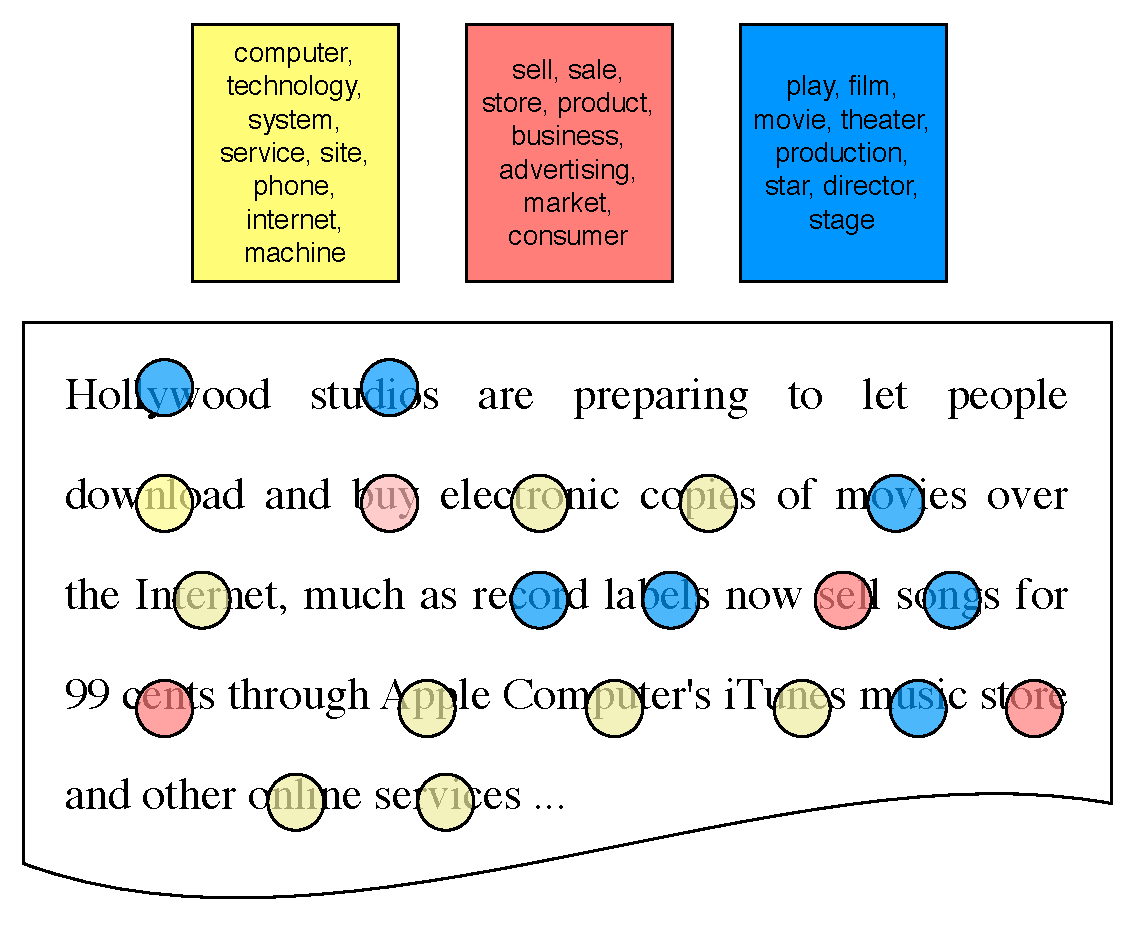
\includegraphics[width=.6\linewidth]{topic_models/inference_3}}
    \only<7>{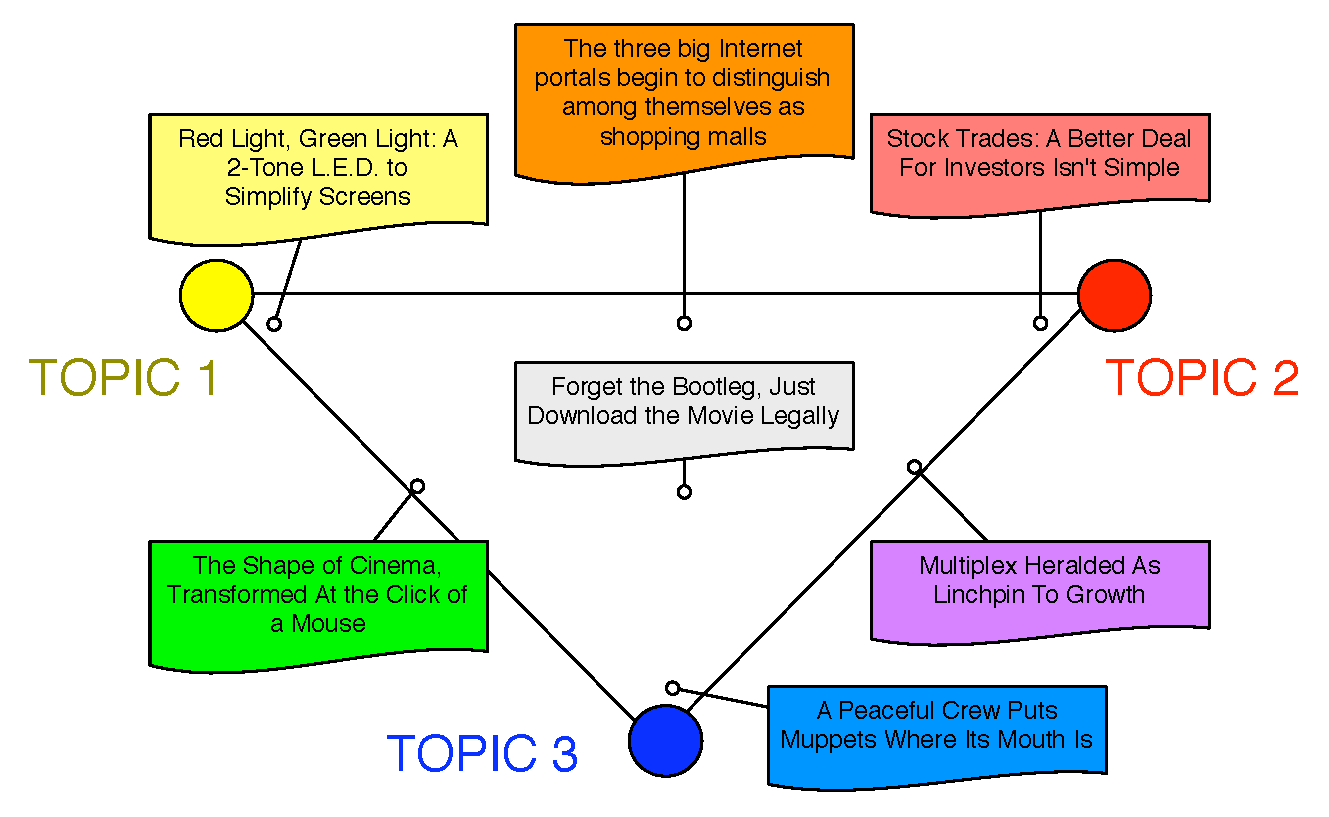
\includegraphics[width=0.9\linewidth]{topic_models/nyt_documents}}
    \only<8>{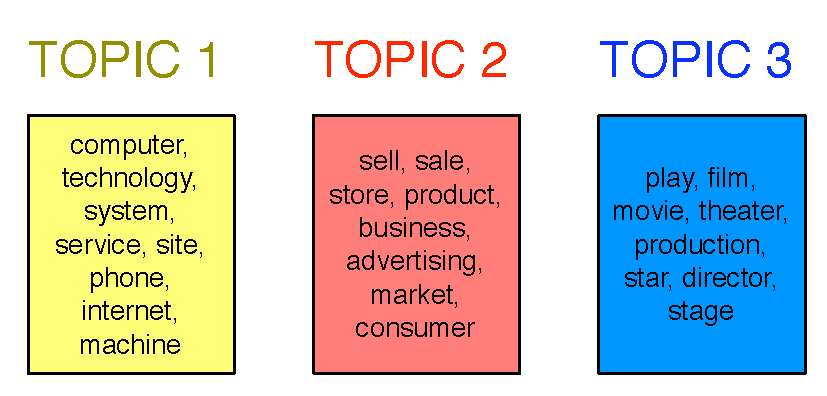
\includegraphics[width=0.9\linewidth]{reading_tea_leaves/figures/nyt_topics_wide}}  
    \only<9>{
    \begin{block}{Inferencer}
        Allows us to apply these topics to another dataset
      \end{block}
    }
  \end{columns}

\end{frame}

\begin{frame}[fragile]
  \frametitle{As Mallet Runs \dots}

  \begin{lstlisting}
<10> LL/token: -10,01271
<20> LL/token: -9,17157
<30> LL/token: -9,01933
<40> LL/token: -8,96692
  \end{lstlisting}

  \begin{itemize}
    \item we want to discover best collection of topics that describes our data
      \item this is defined in terms of probability
        \item stochastic search
          \begin{itemize}
            \item stop when probability levels off
              \item requires thousands of iterations
            \end{itemize}
    \end{itemize}

\end{frame}

\begin{frame}[fragile]
  \frametitle{As Mallet Runs \dots}

  \begin{lstlisting}
0	5	species environmental water natural understanding study research processes climate change ocean global carbon studies production marine important conditions populations effects 
1	5	materials research chemistry properties chemical high magnetic optical surface electron state phase structures structure devices electronic metal molecular studies program 
2	5	systems system design research data control performance network based time applications develop software techniques proposed power application networks developed high 
  \end{lstlisting}

  \begin{itemize}
    \item ID of the topic
    \item Weight of the topic (start the same)
    \item The most probable words in the topic
   \end{itemize}

\end{frame}

\begin{frame}[fragile]
  \frametitle{Word-Topic Association}
  \begin{lstlisting}
0       5       species environmental water natural understanding study research processes climate change ocean global carbon production studies marine populations conditions important long 
1       5       materials research chemistry properties chemical high magnetic optical surface electron phase state structures structure molecular devices electronic metal studies program 
    \end{lstlisting}

    \begin{itemize}
      \item Same information as displayed as Mallet runs
        \item Shows the most probable words in each topic
      \end{itemize}

\end{frame}


\begin{frame}{What topics did we discover?}
\small
  \begin{enumerate}
    \setcounter{enumi}{-1}
    \item {\bf Computer Science}: data performance network software algorithms 
    \item {\bf Students}: students education undergraduate school learning faculty 
    \item {\bf Chemistry}: chemistry chemical organic molecular reactions metal
    \item {\bf Physics}: high observations waves energy time physics stars flow 
    \item {\bf Math}: equations models geometry analysis number mathematics
    \item {\bf Social Science}: social economic information policy human political 
    \item {\bf Earth Science}: water climate ice ocean carbon high models soil sea
    \item {\bf Training}: research support award workshop conference program 
    \item {\bf Biology}: species cell genes plant gene molecular cells dna proteins
    \item {\bf Materials Science}: materials research high properties
      project optical magnetic
    \end{enumerate}
\end{frame}

\begin{frame}[fragile]
  \frametitle{What documents are associated with each topic?}

  \begin{lstlisting}
8724    doc8724 8       0.5295448158189615      0       0.46418192697602284     7
       0.0011271253410239611   ...
8725    doc8725 9       0.8864657651849538      7       0.05057323989491986     2
       0.045321605268636066     ...
        \end{lstlisting}

    \begin{itemize}
      \item Document 8724 is associated with topic 8 and topic 0
        \item These are the Biology and Computer Science topics
      \end{itemize}

      \pause

      \vspace{-3cm}

  \begin{block}{doc8724}
    \small
Humans and other animals use visual  looming  of a stimulus to detect change in distance of a stimulus in the depth of the visual field. It is unclear how such visual cues drive neural signals that guide appropriate behavioral responses such as approach or avoidance for such a stimulus. Results will be important beyond insect vision, for understanding depth detection and obstacle avoidance by visual mechanisms in general, and for developing useful machine vision and guidance systems in robotics for computational neuroscience.
  \end{block}

\end{frame}


%\begin{frame}
%  \frametitle{Applying topics to \textsc{nrc} data}
%  \begin{itemize}
%    \item Assume that we are satisfied with this topic analysis
%    \item \textsc{nsf} is convenient example
%      \begin{itemize}
%        \item \textsc{eu}-wide research
%        \item Wikipedia
%        \item Publications
%      \end{itemize}
%      \item Associate \alert<2>{new documents} with some \alert<3>{standard}
%      \item Compare funding levels for comparable topics (regardless of internal classification)
%  \end{itemize}
%
%\end{frame}
%
%
%\begin{frame}
%  \frametitle{Applying Topics}
%    \begin{block}{Mallet Command}
%      mallet infer-topics --input \alert<2>{nrc.mallet} --inferencer \alert<3>{nsf\_10.inf} --output-doc-topics \alert<4>{nrc.doc}
%    \end{block}
%
%    \begin{itemize}
%      \item Document to apply model to
%      \item Inferencer created from model
%      \item Output file
%    \end{itemize}
%
%\end{frame}
%
%
%\begin{frame}[fragile]
%
%\frametitle{Finding Similar Articles}
%
%  \begin{itemize}
%    \item We found a computational biology grant from \textsc{nsf}
%    \item How do we find similar grants in \textsc{nrc}?
%    \item Look for grants with high probability for Topic 0 and Topic 8
%  \end{itemize}
%
%      \begin{lstlisting}
%187     pages/1253988731023     8       0.4546086322042478      0       0.3405459548
%4236727     5       0.13293471300185633     ...
%186     pages/1253988731014     8       0.41662982704829793     9       0.1797146162
%3145737     ...
%0981687477E-4   
%148     pages/1253984734617     8       0.502404238103382       0       0.4069265225
%375647      6       0.050378383174511626    ...
%      \end{lstlisting}
%
%      \pause
%      \vspace{-3cm}
%
%      \begin{block}{Look it up \dots}
%        \centering
%        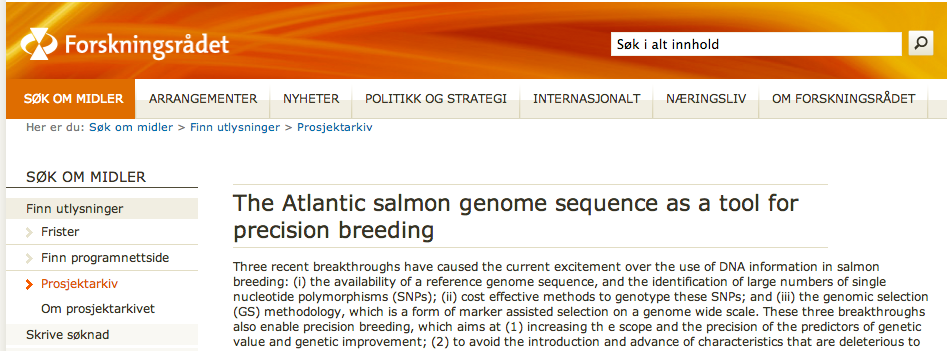
\includegraphics[width=0.8\linewidth]{topic_models/nrc_lookup}
%      \end{block}
%
%\end{frame}

\begin{frame}
  \frametitle{Which topics appear together?}
  \centering
    \only<1>{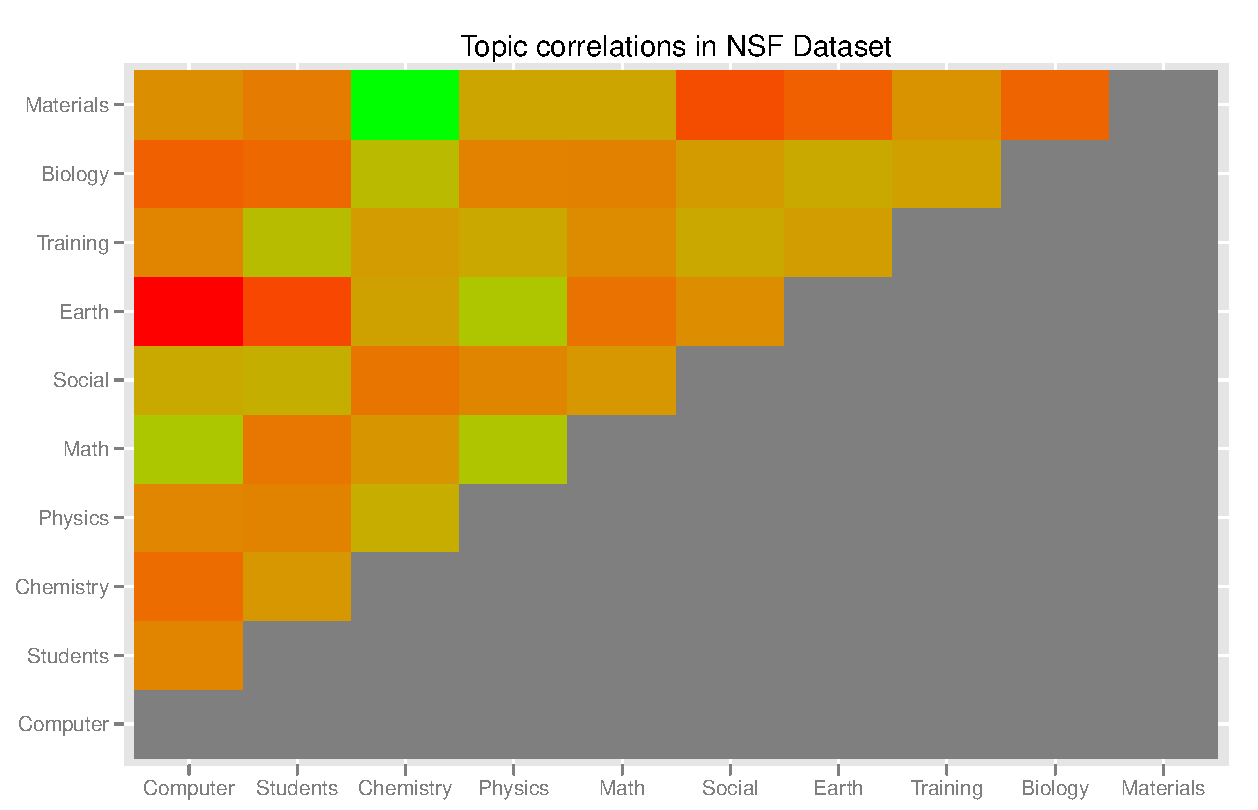
\includegraphics[width=.8\linewidth]{topic_models/nsf_cor}}
%    \only<2>{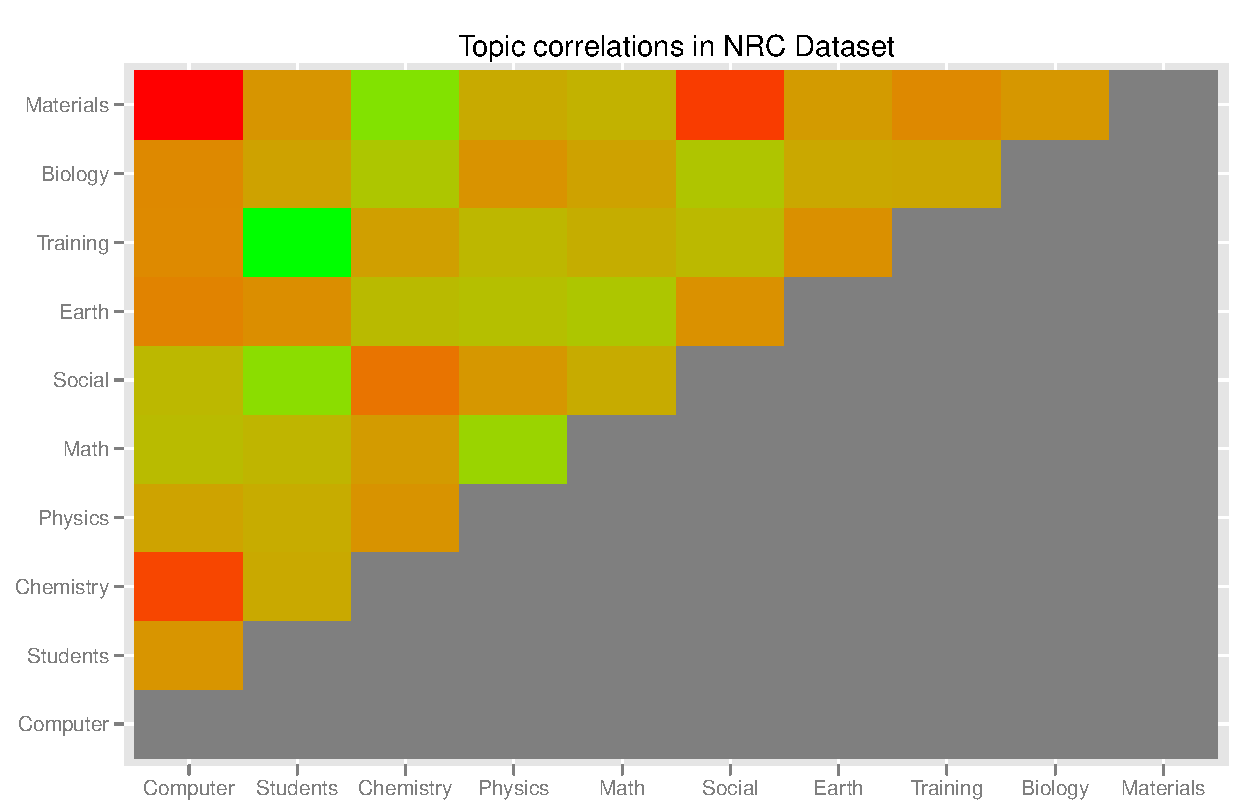
\includegraphics[width=.8\linewidth]{topic_models/nrc_cor}}
\end{frame}

\begin{frame}
  \frametitle{Much more to be done!}

  \begin{itemize}
    \item Bigrams: not all strings separated by spaces are words
      \begin{itemize}
        \item high energy, nano materials, seismic models, undergraduate students
          \item need to be discovered along with topics
        \end{itemize}
        \item Choosing correct granularity
        \item Refining stopword list: investigator, study, research
        \item \alert<2>{Adding constraints}
        \item \alert<2>{Multiple languages}
   \end{itemize}

\end{frame}